\documentclass[11pt,a4paper]{article}

% ---------------------------------------------------------------------------
% Build:  bash scripts/paper/build_pdf.sh   (from the repository root)
% Tables: paper/tables/*.tex from scripts/paper/make_tables.py
% Figures: paper/figures/*.pdf from scripts/paper/make_figures.py
% ---------------------------------------------------------------------------

\usepackage[T1]{fontenc}
\usepackage[utf8]{inputenc}
\usepackage[margin=1in]{geometry}
\usepackage{times}
\usepackage[htt]{hyphenat}
\usepackage{microtype}
\usepackage{array}
\usepackage{booktabs}
\usepackage{graphicx}
\usepackage{amsmath}
\usepackage{amssymb}
\usepackage{xcolor}
\usepackage{caption}
\usepackage{subcaption}
\usepackage{enumitem}
\usepackage[hidelinks]{hyperref}
\hypersetup{
  pdftitle={Independent Retrieval Does Not Reduce False Endorsement on SciFact},
  pdfauthor={Rushi Balapure},
  pdfsubject={Scientific claim verification, independent retrieval, abstention, negative result},
  pdfkeywords={fact checking, scientific claims, retrieval, abstention, reproducibility}
}
\usepackage{natbib}

\setlength{\emergencystretch}{3em}

% Generated by scripts/paper/make_tables.py. Do not edit by hand.
\newcommand{\lunadevBZeron}{300}
\newcommand{\lunadevBZeromicroFOne}{0.557}
\newcommand{\lunadevBZeromacroFOne}{0.517}
\newcommand{\lunadevBZerofe}{0.448}
\newcommand{\lunadevBZerosupportRecall}{0.872}
\newcommand{\lunadevBZerofailclosed}{0}
\newcommand{\lunadevBZerosupportPrecision}{0.554}
\newcommand{\lunadevBZeroneiPrecision}{0.467}
\newcommand{\lunadevBOnen}{300}
\newcommand{\lunadevBOnemicroFOne}{0.840}
\newcommand{\lunadevBOnemacroFOne}{0.838}
\newcommand{\lunadevBOnefe}{0.049}
\newcommand{\lunadevBOnesupportRecall}{0.838}
\newcommand{\lunadevBOnefailclosed}{0}
\newcommand{\lunadevBOnesupportPrecision}{0.916}
\newcommand{\lunadevBOneneiPrecision}{0.802}
\newcommand{\lunadevBTwon}{300}
\newcommand{\lunadevBTwomicroFOne}{0.747}
\newcommand{\lunadevBTwomacroFOne}{0.755}
\newcommand{\lunadevBTwofe}{0.011}
\newcommand{\lunadevBTwosupportRecall}{0.530}
\newcommand{\lunadevBTwofailclosed}{0}
\newcommand{\lunadevBTwosupportPrecision}{0.969}
\newcommand{\lunadevBTwoneiPrecision}{0.628}
\newcommand{\lunadevBThreen}{300}
\newcommand{\lunadevBThreemicroFOne}{0.790}
\newcommand{\lunadevBThreemacroFOne}{0.787}
\newcommand{\lunadevBThreefe}{0.055}
\newcommand{\lunadevBThreesupportRecall}{0.795}
\newcommand{\lunadevBThreefailclosed}{0}
\newcommand{\lunadevBThreesupportPrecision}{0.903}
\newcommand{\lunadevBThreeneiPrecision}{0.740}
\newcommand{\lunadevVDOnen}{268}
\newcommand{\lunadevVDOnemicroFOne}{0.743}
\newcommand{\lunadevVDOnemacroFOne}{0.745}
\newcommand{\lunadevVDOnefe}{0.019}
\newcommand{\lunadevVDOnesupportRecall}{0.598}
\newcommand{\lunadevVDOnefailclosed}{32}
\newcommand{\lunadevVDOnesupportPrecision}{0.955}
\newcommand{\lunadevVDOneneiPrecision}{0.638}
\newcommand{\lunadevVn}{268}
\newcommand{\lunadevVmicroFOne}{0.675}
\newcommand{\lunadevVmacroFOne}{0.673}
\newcommand{\lunadevVfe}{0.000}
\newcommand{\lunadevVsupportRecall}{0.383}
\newcommand{\lunadevVfailclosed}{32}
\newcommand{\lunadevVsupportPrecision}{1.000}
\newcommand{\lunadevVneiPrecision}{0.560}
\newcommand{\lunadevOn}{300}
\newcommand{\lunadevOmicroFOne}{0.857}
\newcommand{\lunadevOmacroFOne}{0.860}
\newcommand{\lunadevOfe}{0.016}
\newcommand{\lunadevOsupportRecall}{0.735}
\newcommand{\lunadevOfailclosed}{0}
\newcommand{\lunadevOsupportPrecision}{0.966}
\newcommand{\lunadevOneiPrecision}{0.756}
\newcommand{\lunadevfediff}{-0.012}
\newcommand{\lunadevfeci}{[-0.031, 0.000]}
\newcommand{\lunadevnpaired}{268}
\newcommand{\lunadevnfamilies}{226}
\newcommand{\lunarerunBZeron}{300}
\newcommand{\lunarerunBZeromicroFOne}{0.547}
\newcommand{\lunarerunBZeromacroFOne}{0.508}
\newcommand{\lunarerunBZerofe}{0.448}
\newcommand{\lunarerunBZerosupportRecall}{0.863}
\newcommand{\lunarerunBZerofailclosed}{0}
\newcommand{\lunarerunBZerosupportPrecision}{0.552}
\newcommand{\lunarerunBZeroneiPrecision}{0.485}
\newcommand{\lunarerunBOnen}{300}
\newcommand{\lunarerunBOnemicroFOne}{0.843}
\newcommand{\lunarerunBOnemacroFOne}{0.842}
\newcommand{\lunarerunBOnefe}{0.044}
\newcommand{\lunarerunBOnesupportRecall}{0.829}
\newcommand{\lunarerunBOnefailclosed}{0}
\newcommand{\lunarerunBOnesupportPrecision}{0.924}
\newcommand{\lunarerunBOneneiPrecision}{0.803}
\newcommand{\lunarerunBTwon}{300}
\newcommand{\lunarerunBTwomicroFOne}{0.747}
\newcommand{\lunarerunBTwomacroFOne}{0.753}
\newcommand{\lunarerunBTwofe}{0.011}
\newcommand{\lunarerunBTwosupportRecall}{0.573}
\newcommand{\lunarerunBTwofailclosed}{0}
\newcommand{\lunarerunBTwosupportPrecision}{0.971}
\newcommand{\lunarerunBTwoneiPrecision}{0.635}
\newcommand{\lunarerunBThreen}{300}
\newcommand{\lunarerunBThreemicroFOne}{0.800}
\newcommand{\lunarerunBThreemacroFOne}{0.795}
\newcommand{\lunarerunBThreefe}{0.049}
\newcommand{\lunarerunBThreesupportRecall}{0.812}
\newcommand{\lunarerunBThreefailclosed}{0}
\newcommand{\lunarerunBThreesupportPrecision}{0.913}
\newcommand{\lunarerunBThreeneiPrecision}{0.764}
\newcommand{\lunarerunVDOnen}{300}
\newcommand{\lunarerunVDOnemicroFOne}{0.757}
\newcommand{\lunarerunVDOnemacroFOne}{0.757}
\newcommand{\lunarerunVDOnefe}{0.016}
\newcommand{\lunarerunVDOnesupportRecall}{0.632}
\newcommand{\lunarerunVDOnefailclosed}{0}
\newcommand{\lunarerunVDOnesupportPrecision}{0.961}
\newcommand{\lunarerunVDOneneiPrecision}{0.643}
\newcommand{\lunarerunVn}{300}
\newcommand{\lunarerunVmicroFOne}{0.687}
\newcommand{\lunarerunVmacroFOne}{0.683}
\newcommand{\lunarerunVfe}{0.000}
\newcommand{\lunarerunVsupportRecall}{0.427}
\newcommand{\lunarerunVfailclosed}{0}
\newcommand{\lunarerunVsupportPrecision}{1.000}
\newcommand{\lunarerunVneiPrecision}{0.564}
\newcommand{\lunarerunOn}{300}
\newcommand{\lunarerunOmicroFOne}{0.870}
\newcommand{\lunarerunOmacroFOne}{0.873}
\newcommand{\lunarerunOfe}{0.005}
\newcommand{\lunarerunOsupportRecall}{0.769}
\newcommand{\lunarerunOfailclosed}{0}
\newcommand{\lunarerunOsupportPrecision}{0.989}
\newcommand{\lunarerunOneiPrecision}{0.766}
\newcommand{\lunarerunfediff}{-0.011}
\newcommand{\lunarerunfeci}{[-0.029, 0.000]}
\newcommand{\lunarerunnpaired}{300}
\newcommand{\lunarerunnfamilies}{246}
\newcommand{\lunaheldBTwon}{300}
\newcommand{\lunaheldBTwomicroFOne}{0.760}
\newcommand{\lunaheldBTwomacroFOne}{0.765}
\newcommand{\lunaheldBTwofe}{0.017}
\newcommand{\lunaheldBTwosupportRecall}{0.581}
\newcommand{\lunaheldBTwofailclosed}{0}
\newcommand{\lunaheldBTwosupportPrecision}{0.960}
\newcommand{\lunaheldBTwoneiPrecision}{0.641}
\newcommand{\lunaheldVDOnen}{262}
\newcommand{\lunaheldVDOnemicroFOne}{0.721}
\newcommand{\lunaheldVDOnemacroFOne}{0.715}
\newcommand{\lunaheldVDOnefe}{0.032}
\newcommand{\lunaheldVDOnesupportRecall}{0.585}
\newcommand{\lunaheldVDOnefailclosed}{38}
\newcommand{\lunaheldVDOnesupportPrecision}{0.925}
\newcommand{\lunaheldVDOneneiPrecision}{0.609}
\newcommand{\lunaheldVn}{262}
\newcommand{\lunaheldVmicroFOne}{0.618}
\newcommand{\lunaheldVmacroFOne}{0.599}
\newcommand{\lunaheldVfe}{0.000}
\newcommand{\lunaheldVsupportRecall}{0.368}
\newcommand{\lunaheldVfailclosed}{38}
\newcommand{\lunaheldVsupportPrecision}{1.000}
\newcommand{\lunaheldVneiPrecision}{0.505}
\newcommand{\lunaheldfediff}{-0.013}
\newcommand{\lunaheldfeci}{[-0.033, 0.000]}
\newcommand{\lunaheldnpaired}{262}
\newcommand{\lunaheldnfamilies}{219}
\newcommand{\mmdevBOnen}{300}
\newcommand{\mmdevBOnemicroFOne}{0.863}
\newcommand{\mmdevBOnemacroFOne}{0.856}
\newcommand{\mmdevBOnefe}{0.093}
\newcommand{\mmdevBOnesupportRecall}{0.966}
\newcommand{\mmdevBOnefailclosed}{0}
\newcommand{\mmdevBOnesupportPrecision}{0.869}
\newcommand{\mmdevBOneneiPrecision}{0.978}
\newcommand{\mmdevBTwon}{300}
\newcommand{\mmdevBTwomicroFOne}{0.870}
\newcommand{\mmdevBTwomacroFOne}{0.867}
\newcommand{\mmdevBTwofe}{0.033}
\newcommand{\mmdevBTwosupportRecall}{0.855}
\newcommand{\mmdevBTwofailclosed}{0}
\newcommand{\mmdevBTwosupportPrecision}{0.943}
\newcommand{\mmdevBTwoneiPrecision}{0.847}
\newcommand{\mmdevVDOnen}{300}
\newcommand{\mmdevVDOnemicroFOne}{0.853}
\newcommand{\mmdevVDOnemacroFOne}{0.851}
\newcommand{\mmdevVDOnefe}{0.033}
\newcommand{\mmdevVDOnesupportRecall}{0.829}
\newcommand{\mmdevVDOnefailclosed}{0}
\newcommand{\mmdevVDOnesupportPrecision}{0.942}
\newcommand{\mmdevVDOneneiPrecision}{0.794}
\newcommand{\mmdevVn}{300}
\newcommand{\mmdevVmicroFOne}{0.830}
\newcommand{\mmdevVmacroFOne}{0.837}
\newcommand{\mmdevVfe}{0.016}
\newcommand{\mmdevVsupportRecall}{0.692}
\newcommand{\mmdevVfailclosed}{0}
\newcommand{\mmdevVsupportPrecision}{0.964}
\newcommand{\mmdevVneiPrecision}{0.722}
\newcommand{\mmdevfediff}{-0.016}
\newcommand{\mmdevfeci}{[-0.046, 0.011]}
\newcommand{\mmdevnpaired}{300}
\newcommand{\mmdevnfamilies}{246}
\newcommand{\lunadevBTwoallrowsn}{300}
\newcommand{\lunadevBTwoallrowsmicroFOne}{0.747}
\newcommand{\lunadevBTwoallrowsfe}{0.011}
\newcommand{\lunadevBTwoallrowssupportRecall}{0.530}
\newcommand{\lunadevVallrowsn}{300}
\newcommand{\lunadevVallrowsmicroFOne}{0.640}
\newcommand{\lunadevVallrowsfe}{0.000}
\newcommand{\lunadevVallrowssupportRecall}{0.350}
\newcommand{\lunarerunBTwoallrowsn}{300}
\newcommand{\lunarerunBTwoallrowsmicroFOne}{0.747}
\newcommand{\lunarerunBTwoallrowsfe}{0.011}
\newcommand{\lunarerunBTwoallrowssupportRecall}{0.573}
\newcommand{\lunarerunVallrowsn}{300}
\newcommand{\lunarerunVallrowsmicroFOne}{0.687}
\newcommand{\lunarerunVallrowsfe}{0.000}
\newcommand{\lunarerunVallrowssupportRecall}{0.427}
\newcommand{\lunaheldBTwoallrowsn}{300}
\newcommand{\lunaheldBTwoallrowsmicroFOne}{0.760}
\newcommand{\lunaheldBTwoallrowsfe}{0.017}
\newcommand{\lunaheldBTwoallrowssupportRecall}{0.581}
\newcommand{\lunaheldVallrowsn}{300}
\newcommand{\lunaheldVallrowsmicroFOne}{0.583}
\newcommand{\lunaheldVallrowsfe}{0.000}
\newcommand{\lunaheldVallrowssupportRecall}{0.315}
\newcommand{\mmdevBTwoallrowsn}{300}
\newcommand{\mmdevBTwoallrowsmicroFOne}{0.870}
\newcommand{\mmdevBTwoallrowsfe}{0.033}
\newcommand{\mmdevBTwoallrowssupportRecall}{0.855}
\newcommand{\mmdevVallrowsn}{300}
\newcommand{\mmdevVallrowsmicroFOne}{0.830}
\newcommand{\mmdevVallrowsfe}{0.016}
\newcommand{\mmdevVallrowssupportRecall}{0.692}
\newcommand{\retrievalRecall}{0.85}
\newcommand{\retrievalPrecision}{0.07}
\newcommand{\retrievalOverlap}{0.10}
\newcommand{\retrievalUnique}{0.00}
\newcommand{\retrievalUnjudged}{93}
\newcommand{\retrievalRefuting}{0.17}
\newcommand{\retrievalNClaims}{300}
\newcommand{\retrievalNAnnotated}{179}
\newcommand{\lunadevVlabelstotal}{300}
\newcommand{\lunadevVlabelssupported}{41}
\newcommand{\lunadevVlabelscontradicted}{34}
\newcommand{\lunadevVlabelsunaddressed}{60}
\newcommand{\lunadevVlabelsunderdetermined}{165}
\newcommand{\lunadevVlabelsnei}{225}
\newcommand{\lunadevVlabelsneishare}{0.75}
\newcommand{\lunaheldVlabelstotal}{300}
\newcommand{\lunaheldVlabelssupported}{39}
\newcommand{\lunaheldVlabelscontradicted}{31}
\newcommand{\lunaheldVlabelsunaddressed}{51}
\newcommand{\lunaheldVlabelsunderdetermined}{179}
\newcommand{\lunaheldVlabelsnei}{230}
\newcommand{\lunaheldVlabelsneishare}{0.77}
\newcommand{\mmdevVlabelstotal}{300}
\newcommand{\mmdevVlabelssupported}{84}
\newcommand{\mmdevVlabelscontradicted}{54}
\newcommand{\mmdevVlabelsunaddressed}{59}
\newcommand{\mmdevVlabelsunderdetermined}{103}
\newcommand{\mmdevVlabelsnei}{162}
\newcommand{\mmdevVlabelsneishare}{0.54}
\newcommand{\lunadevBTwoTokensPerCall}{605}
\newcommand{\lunadevVTokensPerCall}{2,579}
\newcommand{\lunaTokenRatio}{6.4}
\newcommand{\lunadevAgreeN}{163}
\newcommand{\lunadevAgreeBTwosAcc}{0.828}
\newcommand{\lunadevAgreeVacc}{0.828}
\newcommand{\lunadevAgreeVnei}{0.540}
\newcommand{\lunadevAgreeNeiCount}{88}
\newcommand{\lunadevAgreeVerrors}{28}
\newcommand{\lunadevNeiOnlyN}{50}
\newcommand{\lunadevNeiOnlyBTwosAcc}{0.600}
\newcommand{\lunadevNeiOnlyVacc}{0.580}
\newcommand{\lunadevNeiOnlyVnei}{1.000}
\newcommand{\lunadevNeiOnlyNeiCount}{50}
\newcommand{\lunadevNeiOnlyVerrors}{21}
\newcommand{\lunadevConflictN}{55}
\newcommand{\lunadevConflictBTwosAcc}{0.618}
\newcommand{\lunadevConflictVacc}{0.309}
\newcommand{\lunadevConflictVnei}{1.000}
\newcommand{\lunadevConflictNeiCount}{55}
\newcommand{\lunadevConflictVerrors}{38}
\newcommand{\lunadevVerrors}{87}
\newcommand{\lunadevVconflictErrors}{38}
\newcommand{\lunadevAgreeUnaddressed}{60}
\newcommand{\lunadevAgreeUnderdetermined}{28}
\newcommand{\lunaheldAgreeN}{139}
\newcommand{\lunaheldAgreeBTwosAcc}{0.871}
\newcommand{\lunaheldAgreeVacc}{0.842}
\newcommand{\lunaheldAgreeVnei}{0.496}
\newcommand{\lunaheldAgreeNeiCount}{69}
\newcommand{\lunaheldAgreeVerrors}{22}
\newcommand{\lunaheldNeiOnlyN}{73}
\newcommand{\lunaheldNeiOnlyBTwosAcc}{0.603}
\newcommand{\lunaheldNeiOnlyVacc}{0.548}
\newcommand{\lunaheldNeiOnlyVnei}{1.000}
\newcommand{\lunaheldNeiOnlyNeiCount}{73}
\newcommand{\lunaheldNeiOnlyVerrors}{33}
\newcommand{\lunaheldConflictN}{50}
\newcommand{\lunaheldConflictBTwosAcc}{0.700}
\newcommand{\lunaheldConflictVacc}{0.100}
\newcommand{\lunaheldConflictVnei}{1.000}
\newcommand{\lunaheldConflictNeiCount}{50}
\newcommand{\lunaheldConflictVerrors}{45}
\newcommand{\lunaheldVerrors}{100}
\newcommand{\lunaheldVconflictErrors}{45}
\newcommand{\lunaheldAgreeUnaddressed}{51}
\newcommand{\lunaheldAgreeUnderdetermined}{18}
\newcommand{\mmdevAgreeN}{214}
\newcommand{\mmdevAgreeBTwosAcc}{0.911}
\newcommand{\mmdevAgreeVacc}{0.925}
\newcommand{\mmdevAgreeVnei}{0.355}
\newcommand{\mmdevAgreeNeiCount}{76}
\newcommand{\mmdevAgreeVerrors}{16}
\newcommand{\mmdevNeiOnlyN}{36}
\newcommand{\mmdevNeiOnlyBTwosAcc}{0.861}
\newcommand{\mmdevNeiOnlyVacc}{0.917}
\newcommand{\mmdevNeiOnlyVnei}{1.000}
\newcommand{\mmdevNeiOnlyNeiCount}{36}
\newcommand{\mmdevNeiOnlyVerrors}{3}
\newcommand{\mmdevConflictN}{50}
\newcommand{\mmdevConflictBTwosAcc}{0.700}
\newcommand{\mmdevConflictVacc}{0.360}
\newcommand{\mmdevConflictVnei}{1.000}
\newcommand{\mmdevConflictNeiCount}{50}
\newcommand{\mmdevConflictVerrors}{32}
\newcommand{\mmdevVerrors}{51}
\newcommand{\mmdevVconflictErrors}{32}
\newcommand{\mmdevAgreeUnaddressed}{59}
\newcommand{\mmdevAgreeUnderdetermined}{17}
\newcommand{\sweepModels}{4}
\newcommand{\sweepClosed}{4}
\newcommand{\sweepOpen}{0}
\newcommand{\sweepLower}{0}
\newcommand{\sweepEqual}{4}
\newcommand{\sweepHigher}{0}
\newcommand{\sweepExcludeZero}{0}
\newcommand{\sweepFOneLower}{4}
\newcommand{\sweepSupportLower}{1}
\newcommand{\sweepRefuteLower}{4}
\newcommand{\sweepRefuteEqual}{0}
\newcommand{\sweepSupportEqual}{3}
\newcommand{\sweepModelsWord}{four}
\newcommand{\sweepClosedWord}{four}
\newcommand{\sweepOpenWord}{none}
\newcommand{\sweepLowerWord}{none}
\newcommand{\sweepEqualWord}{four}
\newcommand{\sweepHigherWord}{none}
\newcommand{\sweepExcludeZeroWord}{none}
\newcommand{\sweepFOneLowerWord}{four}
\newcommand{\sweepSupportLowerWord}{one}
\newcommand{\sweepRefuteLowerWord}{four}
\newcommand{\sweepRefuteEqualWord}{none}
\newcommand{\sweepSupportEqualWord}{three}
\newcommand{\sweepSplit}{all closed-weight}
\newcommand{\sweepAdditional}{3}
\newcommand{\sweepAdditionalWord}{three}
\newcommand{\sweepAdditionalList}{GPT-6 Astra, GPT-6 Sol and GPT-5.6 Terra}
\newcommand{\sweepRoute}{They use the same hosted API as the Luna family, so their cost and token accounting match the Luna family's.}
\newcommand{\sweepRefuteAll}{4}
\newcommand{\sweepRefuteAllWord}{four}
\newcommand{\sweepRefuteSome}{0}
\newcommand{\sweepRefuteSomeWord}{none}
\newcommand{\sweepRefuteNone}{5}
\newcommand{\sweepRefuteNoneWord}{five}
\newcommand{\sweepSupportAll}{0}
\newcommand{\sweepSupportAllWord}{none}
\newcommand{\sweepSupportSome}{1}
\newcommand{\sweepSupportSomeWord}{one}
\newcommand{\sweepSupportNone}{6}
\newcommand{\sweepSupportNoneWord}{six}
\newcommand{\sweepGainedSupport}{1}
\newcommand{\sweepGainedSupportWord}{one}
\newcommand{\sweepGainedRefute}{0}
\newcommand{\sweepGainedRefuteWord}{none}
\newcommand{\sweepAgreeBTwo}{24}
\newcommand{\sweepAgreeBTwoWord}{24}
\newcommand{\sweepAgreeV}{27}
\newcommand{\sweepAgreeVWord}{27}
\newcommand{\sweepRefuteTotal}{9}
\newcommand{\sweepSupportTotal}{7}
\newcommand{\sweepRefuteTotalWord}{nine}
\newcommand{\sweepSupportTotalWord}{seven}
\newcommand{\sweepGainedSupportPhrase}{one model--claim pair}
\newcommand{\sweepGainedRefutePhrase}{no model--claim pair}
\newcommand{\sweepRefuteLowerPhrase}{all four models}
\newcommand{\sweepFOneLowerPhrase}{all four models}
\newcommand{\sweepFEmaxPct}{5\%}
\newcommand{\sweepBTwomin}{0.800}
\newcommand{\sweepBTwomax}{0.867}
\newcommand{\lunadevdiscBTwo}{2}
\newcommand{\lunadevdiscV}{0}
\newcommand{\lunadevmcnemarp}{0.50}
\newcommand{\lunadevnnonsup}{161}
\newcommand{\lunarerundiscBTwo}{2}
\newcommand{\lunarerundiscV}{0}
\newcommand{\lunarerunmcnemarp}{0.50}
\newcommand{\lunarerunnnonsup}{183}
\newcommand{\lunahelddiscBTwo}{2}
\newcommand{\lunahelddiscV}{0}
\newcommand{\lunaheldmcnemarp}{0.50}
\newcommand{\lunaheldnnonsup}{156}
\newcommand{\mmdevdiscBTwo}{5}
\newcommand{\mmdevdiscV}{2}
\newcommand{\mmdevmcnemarp}{0.45}
\newcommand{\mmdevnnonsup}{183}
\newcommand{\feMinDiscordant}{6}
\newcommand{\lunadevRulebtwoacc}{0.743}
\newcommand{\lunadevRulebtwofe}{0.012}
\newcommand{\lunadevRulebtwosupportRecall}{0.523}
\newcommand{\lunadevRulebtworefuteRecall}{0.804}
\newcommand{\lunadevRuleasrunacc}{0.675}
\newcommand{\lunadevRuleasrunfe}{0.000}
\newcommand{\lunadevRuleasrunsupportRecall}{0.383}
\newcommand{\lunadevRuleasrunrefuteRecall}{0.627}
\newcommand{\lunadevRuledzeroacc}{0.683}
\newcommand{\lunadevRuledzerofe}{0.019}
\newcommand{\lunadevRuledzerosupportRecall}{0.430}
\newcommand{\lunadevRuledzerorefuteRecall}{0.686}
\newcommand{\lunadevRuledoneacc}{0.743}
\newcommand{\lunadevRuledonefe}{0.019}
\newcommand{\lunadevRuledonesupportRecall}{0.598}
\newcommand{\lunadevRuledonerefuteRecall}{0.745}
\newcommand{\lunadevRulefallbackacc}{0.750}
\newcommand{\lunadevRulefallbackfe}{0.037}
\newcommand{\lunadevRulefallbacksupportRecall}{0.645}
\newcommand{\lunadevRulefallbackrefuteRecall}{0.804}
\newcommand{\lunaheldRulebtwoacc}{0.763}
\newcommand{\lunaheldRulebtwofe}{0.013}
\newcommand{\lunaheldRulebtwosupportRecall}{0.585}
\newcommand{\lunaheldRulebtworefuteRecall}{0.754}
\newcommand{\lunaheldRuleasrunacc}{0.618}
\newcommand{\lunaheldRuleasrunfe}{0.000}
\newcommand{\lunaheldRuleasrunsupportRecall}{0.368}
\newcommand{\lunaheldRuleasrunrefuteRecall}{0.456}
\newcommand{\lunaheldRuledzeroacc}{0.653}
\newcommand{\lunaheldRuledzerofe}{0.000}
\newcommand{\lunaheldRuledzerosupportRecall}{0.415}
\newcommand{\lunaheldRuledzerorefuteRecall}{0.526}
\newcommand{\lunaheldRuledoneacc}{0.721}
\newcommand{\lunaheldRuledonefe}{0.032}
\newcommand{\lunaheldRuledonesupportRecall}{0.585}
\newcommand{\lunaheldRuledonerefuteRecall}{0.614}
\newcommand{\lunaheldRulefallbackacc}{0.756}
\newcommand{\lunaheldRulefallbackfe}{0.032}
\newcommand{\lunaheldRulefallbacksupportRecall}{0.632}
\newcommand{\lunaheldRulefallbackrefuteRecall}{0.684}
\newcommand{\mmdevRulebtwoacc}{0.870}
\newcommand{\mmdevRulebtwofe}{0.033}
\newcommand{\mmdevRulebtwosupportRecall}{0.855}
\newcommand{\mmdevRulebtworefuteRecall}{0.903}
\newcommand{\mmdevRuleasrunacc}{0.830}
\newcommand{\mmdevRuleasrunfe}{0.016}
\newcommand{\mmdevRuleasrunsupportRecall}{0.692}
\newcommand{\mmdevRuleasrunrefuteRecall}{0.823}
\newcommand{\mmdevRuledzeroacc}{0.847}
\newcommand{\mmdevRuledzerofe}{0.038}
\newcommand{\mmdevRuledzerosupportRecall}{0.769}
\newcommand{\mmdevRuledzerorefuteRecall}{0.919}
\newcommand{\mmdevRuledoneacc}{0.853}
\newcommand{\mmdevRuledonefe}{0.033}
\newcommand{\mmdevRuledonesupportRecall}{0.829}
\newcommand{\mmdevRuledonerefuteRecall}{0.823}
\newcommand{\mmdevRulefallbackacc}{0.873}
\newcommand{\mmdevRulefallbackfe}{0.055}
\newcommand{\mmdevRulefallbacksupportRecall}{0.906}
\newcommand{\mmdevRulefallbackrefuteRecall}{0.919}
\newcommand{\lunaflipsBOne}{10}
\newcommand{\lunaflipsBOnen}{300}
\newcommand{\lunaflipsBOnepct}{3}
\newcommand{\lunaflipsBTwo}{26}
\newcommand{\lunaflipsBTwon}{300}
\newcommand{\lunaflipsBTwopct}{9}
\newcommand{\lunaflipsBThree}{8}
\newcommand{\lunaflipsBThreen}{300}
\newcommand{\lunaflipsBThreepct}{3}
\newcommand{\lunaflipsV}{14}
\newcommand{\lunaflipsVn}{268}
\newcommand{\lunaflipsVpct}{5}
\newcommand{\lunadevVfailsupport}{10}
\newcommand{\lunadevVfailrefute}{11}
\newcommand{\lunadevVfailnei}{11}
\newcommand{\lunaheldVfailsupport}{18}
\newcommand{\lunaheldVfailrefute}{7}
\newcommand{\lunaheldVfailnei}{13}


\setlist[itemize]{leftmargin=1.2em,itemsep=1pt,topsep=3pt}
\setlist[enumerate]{leftmargin=1.4em,itemsep=1pt,topsep=3pt}
\captionsetup{font=small,labelfont=bf}
\newcommand{\ie}{\emph{i.e.}}
\newcommand{\eg}{\emph{e.g.}}
\newcommand{\Dzero}{\ensuremath{D_0}}
\newcommand{\Done}{\ensuremath{D_1}}
\newcommand{\Dunion}{\ensuremath{D_0 \cup D_1}}

\title{\textbf{Independent Retrieval Does Not Reduce False Endorsement on SciFact}}
\author{Rushi Balapure}
\date{}

\begin{document}
\maketitle

\begin{abstract}
False endorsement---predicting SUPPORT when the gold label is not
support---is a costly error in scientific claim checking. We ask whether a
staged pipeline that reconciles the original citations (\Dzero) with
independently retrieved abstracts (\Done) reduces it relative to a
same-evidence, evidence-first baseline (B2). Four isolated, fail-closed
roles run as stateless calls to one model.

On 300 SciFact development claims scored with GPT-6 Luna under a frozen
configuration, B2's false-endorsement rate is \lunadevBTwofe{} and the
validator (V) reaches \lunadevVfe{}. The reduction rests on
\lunadevdiscBTwo{} versus \lunadevdiscV{} discordant pairs (exact McNemar
$p=\lunadevmcnemarp{}$); the 95\% interval
(\lunadevfediff{}, \lunadevfeci{}) includes zero. SUPPORT recall falls from
\lunadevBTwosupportRecall{} to \lunadevVsupportRecall{} (66 missed supported
claims against 19 missed contradictions). A 300-claim held-out run repeats
the pattern, with \lunaheldVfailclosed{} of 300 V requests failing closed.
The independent arm alone (\mbox{V-D1}) endorses \emph{more} falsely than
B2 on that held-out sample (\lunaheldVDOnefe{} against \lunaheldBTwofe{}).
A second model (MiniMax M3.1 Flash) moves in the same direction
(\mmdevBTwofe{} to \mmdevVfe{}; SUPPORT recall \mmdevBTwosupportRecall{} to
\mmdevVsupportRecall{}), again with an interval covering zero.

Independent retrieval finds no annotated document that was not already
cited (unique yield \retrievalUnique{}). Most V errors come from
disagreement between the two scopes, which the reconciler maps to
underdetermined by construction. V is more conservative than B2, not more
accurate, and this corpus cannot test whether independent retrieval
repairs a wrong citation.
\end{abstract}

\noindent\textbf{Artifact.} Every table and figure is generated from saved
prediction files by \texttt{scripts/paper/}. The corpus, splits, prompts,
and configurations are in the accompanying repository
(Appendix~\ref{app:repro}). The primary development and held-out runs use
the same frozen configuration; a later re-run of the development sample
after a retry policy was added is reported as a second run, not as the
primary result.

\section{Introduction}

A claim checker that reads only the citations offered with a claim
inherits the generator's evidence. If those citations are wrong, or
support a slightly different claim, the checker cannot notice. One
proposed remedy is independent retrieval: search again, judge the new
passages separately, and reconcile the two scopes. Recent work on
search-augmented factuality evaluation \citep{wei2024longform}, self-check
agents \citep{march2026,hirsch2026blame}, and retrieval-augmented
verifiers \citep{yue2024rafts,zheng2024rav} points in that direction.
The assumption is rarely tested against a same-evidence control on
scientific claims, where the original citations are often correct and
where abstention can be the right answer.

We build a staged validator (\textbf{V}) that separates four roles---a
sealed claim-blind reader, a claim-visible judge over four labels, a
citation auditor over the original references, and a reconciler---across
two evidence scopes: the original citations (\Dzero) and independently
retrieved abstracts (\Done). The comparison is against a same-evidence
baseline (\textbf{B2}) that reads a neutral question over the original
citations in an isolated reader and then compares. B2 is the
evidence-first control, not the strongest same-evidence configuration we
ran: a claim-visible judge over the same citations (B1) has higher
micro-F1.

The specified primary outcome is false endorsement: the rate at which a
method predicts SUPPORT for a claim whose gold label is not support.
The observed answer is inconclusive. On the frozen development sample the
paired difference between V and B2 is \lunadevfediff{}
(\lunadevfeci{}), which includes zero, and an exact McNemar test on the
\lunadevdiscBTwo{} versus \lunadevdiscV{} discordant pairs gives
$p=\lunadevmcnemarp{}$. The held-out sample repeats the pattern. V
reaches zero false endorsements on both Luna samples by withholding
support: SUPPORT recall drops from \lunadevBTwosupportRecall{} to
\lunadevVsupportRecall{} on development, and on the held-out sample
\lunaheldVfailclosed{} of 300 claims fail closed. Both false endorsement
and support recall are needed to judge the trade-off.

Three observations frame the result.

\begin{itemize}
  \item \textbf{This corpus cannot test the motivating mechanism.} In
    SciFact the annotated gold documents are a subset of the cited
    documents, so independent retrieval's unique yield is
    \retrievalUnique{}. The experiment measures what happens when a
    second reader of the same literature is added to gold citations, not
    whether search repairs a wrong citation.
  \item \textbf{The conservatism is a reconciliation policy, not a
    retrieval gain.} When the two four-way labels agree, V matches B2.
    When they differ on the scored three-way label, V abstains by
    construction and is right only as often as those claims are gold NEI.
    About half of the recorded ``conflicts'' are
    unaddressed-versus-underdetermined: both scopes already say NEI.
  \item \textbf{The cost of that policy is missed support.} On the full
    development sample V misses 66 supported claims and 19 contradicted
    ones. A thirty-claim subset of four closed-weight models from one
    vendor lineage concentrates the loss on REFUTE; that subset does not
    match the full-sample class breakdown and is not a replication.
\end{itemize}

The contribution is a reproducible measurement of what independent
retrieval and evidence-first staging do, and do not do, on SciFact,
together with the artifact that makes the measurement checkable. We
report it as an inconclusive result with a mechanism, not as evidence
that independent retrieval does not help in general.

\section{Related Work}

\subsection{Scientific claim verification}

FEVER \citep{thorne2018fever} established the claim--evidence format this
paper follows; FEVEROUS \citep{aly2021feverous} extended it to mixed
evidence. SciFact \citep{wadden2020scifact} pairs scientific claims with
abstracts and rationale sentences and supplies support, refute, and
not-enough-information labels. Official SciFact systems are
retrieval-plus-rationale pipelines scored at the abstract and sentence
level: VeriSci is the original cascade in that paper, and MultiVerS
\citep{wadden2022multivers} is the usual supervised reference (about 72.5
abstract-level label-only F1). Those numbers are not interchangeable with
the claim-level three-way micro-F1 we report. SciFact-Open
\citep{wadden2022scifactopen} extends the task to open-domain retrieval;
we use a frozen corpus only. Missci \citep{glockner2024missci} and
RAGTruth \citep{niu2024ragtruth} sit at neighbouring boundaries
(fallacy reconstruction; context faithfulness), not as scored
competitors.

LLM-only scientific verification is no longer empty. Alvarez et
al.~\citep{alvarez2024zeroshot} show that GPT-4 few-shot prompting on
citance--abstract pairs is close to MultiVerS under the official SciFact
metrics. TripleCheck \citep{gonzalez2025triplecheck} reports 0.70
claim-level F1 on SciFact development in a zero-shot setting. SciClaims
\citep{ortega2025sciclaims} is an end-to-end generative biomedical
pipeline. We do not reproduce these systems; we cite them so that a
prompt-level B2/V comparison is not mistaken for the only LLM result on
SciFact. Vladika and Matthes \citep{vladika2024knowledge} compare
knowledge sources for open-domain scientific verification and motivate
asking whether a different evidence source changes verdicts.

\subsection{LLM verifiers, retrieval, and citation}

Chain-of-Verification \citep{dhuliawala2024cove} isolates verification
questions from a draft answer; B2 deliberately imitates that isolation
over the original citations. SAFE \citep{wei2024longform} verifies atomic
facts with search and is the reference point for the independent-retrieval
arm. The primitive the judge implements---is this statement supported by
these documents?---is a standard LLM-as-a-judge operation
\citep{zheng2023llmasjudge}. FActScore \citep{min2023factscore} and
MiniCheck \citep{tang2024minicheck} score generated text against grounding
documents; we check an already-atomic scientific claim against retrieved
abstracts, so we inherit the isolation idea and not the metric.
Self-checking agents such as MARCH \citep{march2026,march2026code} add
information separation between proposer and checker. Blame-localization
work \citep{hirsch2026blame} attributes citation errors in a trace; we
evaluate final conclusions and cite that work as the reason not to claim
trace-level credit. RAFTS \citep{yue2024rafts} is a retrieval-then-judge
verifier; RAV \citep{zheng2024rav} is a trained FEVER pipeline whose
thesis is that retrieval quality dominates, which is closer to our
negative retrieval finding than to our staging story. Citation adequacy
is its own evaluation problem \citep{gao2023alce}; our auditor rates each
\Dzero{} citation but we do not report an ALCE-style citation-precision
number.

When two evidence scopes disagree, the model is in a knowledge-conflict
regime. Xie et al.~\citep{xie2024chameleon} show that models follow
coherent external evidence but revert to a parametric prior when some of
the context agrees with that prior; ClashEval \citep{wu2024clasheval}
quantifies the same tug-of-war. The reconciler's default to
underdetermined is a conservative policy in that literature, not a new
theory of conflict.

\subsection{Abstention and selective use}

The precision--coverage curve we plot is the risk--coverage trade-off of
selective classification \citep{elyaniv2010selective,geifman2017selective}:
a reject option that trades coverage for lower error among accepted
claims. Feng et al.~\citep{feng2024abstain} study when an LLM should
abstain because of a knowledge gap; Yang
\citep{yang2026calibratedselective} is a concurrent fact-checking
application. Neither paper is the formalism. Calibration theory
\citep{guo2017calibration} distinguishes verbalised confidence from a
probability fitted on held-out data; we fit a temperature only for the
one condition that verbalises confidence (B1) and do not treat that as a
result for V. We keep a scientific ``underdetermined'' verdict and a
system-level ``defer'' action in separate fields.

\section{Problem Formulation}

\subsection{Inputs and evidence scopes}

Let $c$ be an atomic scientific claim. A claim carries a source span, a
normalised statement, and a \emph{neutral question}: a single
interrogative that preserves population, comparator, units, and causal
scope but does not contain the asserted answer. Two evidence scopes are
available:

\begin{itemize}
  \item $\Dzero$ --- the documents the original report cited. A judgment
    over $\Dzero$ answers: \emph{is the original citation set faithful to
    the claim?}
  \item $\Done$ --- documents retrieved independently from a frozen
    corpus using the neutral question, with the asserted answer, the
    report, and $\Dzero$ hidden. A judgment over $\Done$ answers:
    \emph{what does independent retrieval establish?}
\end{itemize}

A verdict is always relative to a stated scope, corpus, and search
budget. In SciFact the ``original citations'' are the benchmark's cited
documents, which contain the annotated gold evidence. That is a property
of the test bed, not of a generator that might have cited the wrong
paper.

\subsection{Four labels}

Internally the system uses four labels, defined relative to a specified
evidence collection:

\begin{description}[leftmargin=1.1em,style=nextline]
  \item[Supported] Relevant evidence establishes the scoped assertion and
    no unresolved material counterevidence remains in the reviewed pool.
  \item[Contradicted] Relevant evidence establishes an incompatible
    assertion.
  \item[Unaddressed] No reviewed relevant passage answers the claim under
    the stated corpus and retrieval budget.
  \item[Underdetermined] Relevant evidence exists, but disagreement,
    imprecision, or an unsupported inference prevents resolution.
\end{description}

SciFact's native label space is three-way, so the scored mapping is
supported $\to$ SUPPORT, contradicted $\to$ REFUTE, and unaddressed or
underdetermined $\to$ NEI. The four-way distinction is reported but not
scored against gold.

\subsection{Research questions}

\begin{itemize}
  \item \textbf{RQ1 (primary).} Does independent retrieval plus staged
    evidence-first judgment reduce false endorsement relative to
    same-evidence checking? (Specified before the held-out run; not
    publicly registered. The comparison is not compute-matched.)
  \item \textbf{RQ2 (descriptive).} How often do the two scopes disagree,
    and how often does the system defer?
  \item \textbf{RQ3 (deferred).} Do evidence-linked explanations help
    non-experts? No participant was recruited; Appendix~\ref{app:human-study}
    records the unused protocol.
\end{itemize}

\section{System}

Figure~\ref{fig:architecture} shows the two evidence lanes. Roles are
isolated functions with typed inputs; several roles may call the same
model in separate stateless requests. Separate roles do not imply
statistically independent errors.

\begin{figure}[t]
\centering
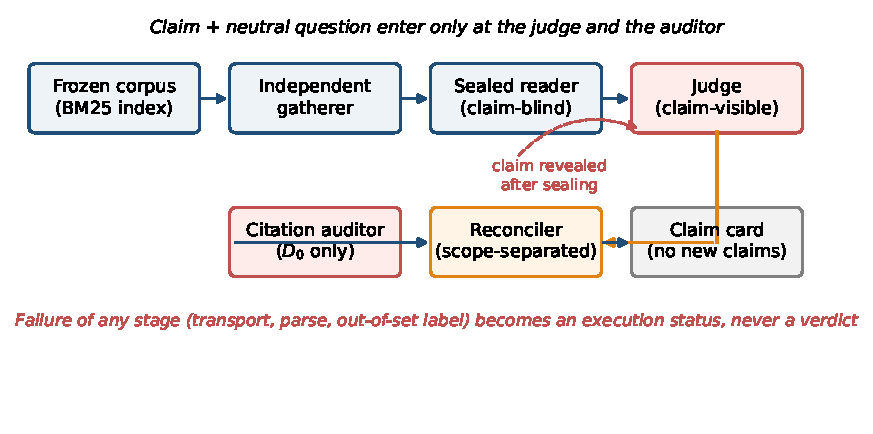
\includegraphics[width=\textwidth]{paper/figures/architecture.pdf}
\caption{The staged validator. The \Done{} lane retrieves and reads from
the neutral question; the claim enters that lane only after the reader's
record is sealed. The \Dzero{} lane judges the original citations alone.
The reconciler keeps a shared label or reports underdetermined. Any
transport or parse failure is an execution status, never a scientific
verdict.}
\label{fig:architecture}
\end{figure}

\begin{description}[leftmargin=1.1em,style=nextline]
  \item[Independent gatherer.] Given the neutral question, retrieves from
    the frozen abstract corpus. Three query forms are issued; the top
    candidates are merged and at most eight passages are kept.
  \item[Evidence reader.] Answers the neutral question from the shuffled
    passages and cites the identifiers it used. Its record is sealed
    before the claim is revealed.
  \item[Judge.] Sees the claim, the sealed record, and the passages, and
    assigns one of the four labels.
  \item[Citation auditor.] Judges the claim against $\Dzero$ alone. It
    never sees $\Done$.
  \item[Reconciler.] If the two four-way labels agree, that label is
    kept; otherwise the verdict is underdetermined. A claim can be
    unsupported by its own citation and supported elsewhere; the two
    facts are reported separately and are not repaired into one score.
\end{description}

The blinding is partial: a neutral question still reveals the topic. The
isolation guarantee is structural (payload shape plus tests), not
semantic. The evaluation scores crowd-sourced SciFact claims, not claims
proposed from a generated report, so the proposer and the renderer are
described in the repository and are not part of the scored comparison.

The system fails closed. A malformed response, a cited identifier that
was not supplied, or an endpoint failure is recorded as
\texttt{failed} or \texttt{timeout} and excluded from scored metrics.
Failed rows are never remapped into a scientific verdict in the primary
accounting. A stricter all-rows accounting that scores those rows as the
conservative NEI is reported as sensitivity. The primary development and
held-out runs do not retry a failed claim. A later development re-run
retries up to four times; it is a second run, not a replacement
(Section~\ref{sec:second-run}).

\section{Experimental Setup}

\subsection{Data and splits}

We use SciFact \citep{wadden2020scifact}. The corpus is the released set
of biomedical abstracts, frozen by hash. Official test labels are not
used. Two samples of 300 claims are frozen by manifest: a development
sample drawn with a fixed seed from the training pool
(\texttt{dev300\_seed42.json}), used for prompt decisions, and SciFact's
public development split, held out locally and used once under the freeze
record. Both samples group claims by cited-document family so that
paraphrases do not straddle the comparison. The scored unit is a
claim-level three-way label, not the official abstract-level or
sentence-level SciFact decision.

SciFact has been public since 2020 and is a plausible pretraining
contaminant \citep{jacovi2023contamination}. Condition B0 (claim only, no
evidence) is the only check on parametric leakage; we do not run a
membership test.

\subsection{Conditions}

All conditions share the frozen corpus, the claim sample, the scoring
code, and the prompt files. They differ in the intervention named in
Table~\ref{tab:conditions}.

\begin{table}[t]
\centering
\caption{The condition matrix. ``Adaptation'' means a prompt-level
implementation of the named mechanism, never a reproduction of a trained
system. V-D1 is recovered from the V predictions by a mapping step, so it
inherits V's execution failures.}
\label{tab:conditions}
\begin{tabular}{lll}
\toprule
ID & Condition & Evidence and reading policy \\
\midrule
B0 & Prior-knowledge judge & No evidence; claim only \\
B1 & Atomic claim, claim-visible judge & $\Dzero$; claim-visible \\
B2 & Neutral question, isolated reader, compare & $\Dzero$; evidence-first \\
B3 & Fresh retrieval, direct judge & $\Done$; claim-visible \\
V-D1 & Fresh retrieval, isolated reader, judge & $\Done$; evidence-first \\
V & Full staged validator & $\Dunion$; reconciled \\
O & Evidence oracle (diagnostic) & Gold rationale sentences \\
\bottomrule
\end{tabular}
\end{table}

B2 is the evidence-first control specified for RQ1. It is not matched to
V on inputs: B2's compare step sees the claim and the sealed reader
record and emits a three-way label; V's judge also sees the passages and
emits a four-way label. It is not matched on compute: V issues three
calls per claim against B2's two, at about \lunaTokenRatio{} times the
tokens. A planned self-consistency control at matched tokens was not
run.

\subsection{Metrics and statistics}

Verification quality is measured by per-class precision, recall and F1,
plus micro and macro F1, on the native three-way label space. The
primary metric is false endorsement: false SUPPORT predictions divided
by the number of gold non-support claims. Coverage is the fraction of
submitted claims that produced a scored prediction; fail-closed rows are
counted.

The specified primary comparison is V versus B2 on false endorsement.
The interval is a paired cluster bootstrap over cited-document families,
2000 resamples, 95\% percentile interval; a claim enters only when both
methods produced an execution-ok, gold-labelled row. Because V's false
endorsement is zero, that interval's upper bound is pinned at zero. We
therefore also report the exact two-sided McNemar test on the discordant
pairs (B2 endorses and V does not, versus the reverse). With a baseline
rate of about 1\%, an exact McNemar test needs at least
\feMinDiscordant{} one-sided discordant events to reach $p<0.05$; the
study was not powered for that. Secondary comparisons are exploratory.
A Holm adjustment was computed on a family of one and is not reported.

\subsection{Models}

GPT-6 Luna is a hosted instruction-tuned model accessed through an
OpenAI-compatible chat endpoint; it is the model behind the primary
comparison, the held-out run, and the cost accounting. MiniMax M3.1
Flash is a second, architecturally unrelated model accessed through a
local agent runtime exposed as a loopback chat endpoint, one fresh
session per request. A fixed agent preamble is prepended to every MiniMax
request, so its token counts are not comparable with Luna's and we do
not report them. Temperature $0$ is requested where the endpoint accepts
it; the hosted OpenAI-compatible path used for Luna omits the field.
Prompts are versioned text files under \texttt{prompts/}; their hashes
enter the freeze record.

A thirty-claim subset of the development sample (ten SUPPORT, ten REFUTE,
ten NEI, seed 42, selected before any sweep model was run) was reused
with four closed-weight models from the same vendor lineage, including
Luna. Open-weight models were attempted through free endpoints; none
completed both conditions, so they contribute no row.

\subsection{Protocol}

The freeze record (\path{docs/freeze.json}, committed 2026-09-26) locks
the model identifier, the corpus hash, and per-method configuration and
prompt hashes. It was written from completed development sidecars after
the development outcome was known, and it is not a public
preregistration. The held-out run (2026-09-25) uses that frozen
configuration and was not retried. The primary development numbers in
this paper are the 2026-09-25 run under the same configuration. On
2026-10-20 the development sample was re-run after a retry policy was
added; that re-run has a different configuration hash, recovered V's
\lunadevVfailclosed{} failed claims, and flipped
\lunaflipsBTwo{} of \lunaflipsBTwon{} B2 labels
(\lunaflipsBTwopct{}\%). We report it as a second run
(Section~\ref{sec:second-run}).

\section{Results}

\subsection{Primary comparison}

Table~\ref{tab:main-dev} gives the development results,
Table~\ref{tab:main-held} the held-out results, and
Table~\ref{tab:paired} the specified paired comparison with an exact
McNemar test. On the frozen Luna development sample, B2 reaches micro-F1
\lunadevBTwomicroFOne{} with false endorsement \lunadevBTwofe{}, while V
reaches micro-F1 \lunadevVmicroFOne{} with false endorsement
\lunadevVfe{} on \lunadevVn{} scored claims
(\lunadevVfailclosed{} fail-closed). The paired difference is
\lunadevfediff{} (\lunadevfeci{}) over \lunadevnpaired{} paired claims;
the interval includes zero. The same comparison on
\lunadevnnonsup{} gold non-support claims is
\lunadevdiscBTwo{} versus \lunadevdiscV{} discordant pairs (exact
McNemar $p=\lunadevmcnemarp{}$). The held-out sample is
\lunahelddiscBTwo{} versus \lunahelddiscV{}
($p=\lunaheldmcnemarp{}$) with interval \lunaheldfediff{}
(\lunaheldfeci{}). MiniMax is \mmdevdiscBTwo{} versus
\mmdevdiscV{} ($p=\mmdevmcnemarp{}$). In every row the data are
compatible with both no reduction and a reduction of a few points. That
is an underpowered comparison, not a demonstration of no effect.

\begin{table}[t]
\centering
\caption{Development sample ($n=300$ claims). FE is false endorsement on
the gold non-support denominator. Fail-closed rows are excluded from the
scored metrics and accounted for in Table~\ref{tab:sensitivity}. Luna
rows are the frozen-configuration run; MiniMax is a later development
run of a second model.}
\label{tab:main-dev}
\footnotesize
\setlength{\tabcolsep}{5pt}
\begin{tabular}{@{}lrrrrr@{}}
\toprule
Method & $n$ & micro-F1 & macro-F1 & FE & SUPPORT R \\
\midrule
\multicolumn{6}{@{}l}{\emph{GPT-6 Luna}} \\[1pt]
B0 & 300 & 0.557 & 0.517 & 0.448 & 0.872 \\
B1 & 300 & 0.840 & 0.838 & 0.049 & 0.838 \\
B2 & 300 & 0.747 & 0.755 & 0.011 & 0.530 \\
B3 & 300 & 0.790 & 0.787 & 0.055 & 0.795 \\
V-D1 & 268 & 0.743 & 0.745 & 0.019 & 0.598 \\
V & 268 & 0.675 & 0.673 & 0.000 & 0.383 \\
O & 300 & 0.857 & 0.860 & 0.016 & 0.735 \\
\midrule
\multicolumn{6}{@{}l}{\emph{MiniMax M3.1 Flash}} \\[1pt]
B1 & 300 & 0.863 & 0.856 & 0.093 & 0.966 \\
B2 & 300 & 0.870 & 0.867 & 0.033 & 0.855 \\
V-D1 & 300 & 0.853 & 0.851 & 0.033 & 0.829 \\
V & 300 & 0.830 & 0.837 & 0.016 & 0.692 \\
\bottomrule
\end{tabular}

\end{table}

\begin{table}[t]
\centering
\caption{Held-out sample (SciFact public development split, used once).
V-D1 is derived from V and inherits its \lunaheldVfailclosed{}
fail-closed rows.}
\label{tab:main-held}
\begin{tabular}{lrrrrrr}
\toprule
Model family & Method & $n$ scored & micro-F1 & macro-F1 & FE (gold non-sup) & SUPPORT recall \\
\midrule
GPT-6-Luna (API) & B2 (D0, evidence-first) & 300 & 0.760 & 0.765 & 0.017 & 0.581 \\
\addlinespace[2pt]
 & V-D1 (D1, evidence-first) & 262 & 0.721 & 0.715 & 0.032 & 0.585 \\
 & V (D0 $\cup$ D1, reconciled) & 262 & 0.618 & 0.599 & 0.000 & 0.368 \\
\midrule
\bottomrule
\end{tabular}

\end{table}

\begin{table}[t]
\centering
\caption{V versus B2 on false endorsement. ``B2 only'' and ``V only''
are discordant pairs among gold non-support claims. McNemar $p$ is the
exact two-sided test. The percentile bootstrap interval is shown for
continuity with the specified analysis; V's zero FE pins its upper
bound at zero.}
\label{tab:paired}
\footnotesize
\setlength{\tabcolsep}{4.5pt}
\begin{tabular}{@{}llrrrrrl@{}}
\toprule
Model & Run & $n$ & non-supp. & B2 only & V only & McNemar $p$ & $\Delta$FE [95\% CI] \\
\midrule
GPT-6 Luna & development & 268 & 161 & 2 & 0 & 0.50 & -0.012 [-0.031, 0.000] \\
GPT-6 Luna & development, second run & 300 & 183 & 2 & 0 & 0.50 & -0.011 [-0.029, 0.000] \\
GPT-6 Luna & held-out & 262 & 156 & 2 & 0 & 0.50 & -0.013 [-0.033, 0.000] \\
MiniMax M3.1 Flash & development & 300 & 183 & 5 & 2 & 0.45 & -0.016 [-0.046, 0.011] \\
\bottomrule
\end{tabular}

\end{table}

Figure~\ref{fig:falseendorsement} places each completed development
condition by false endorsement and SUPPORT recall. V sits at zero
false endorsement and the lowest support recall. B1, not B2, is the
highest-F1 same-evidence cell.

\begin{figure}[t]
\centering
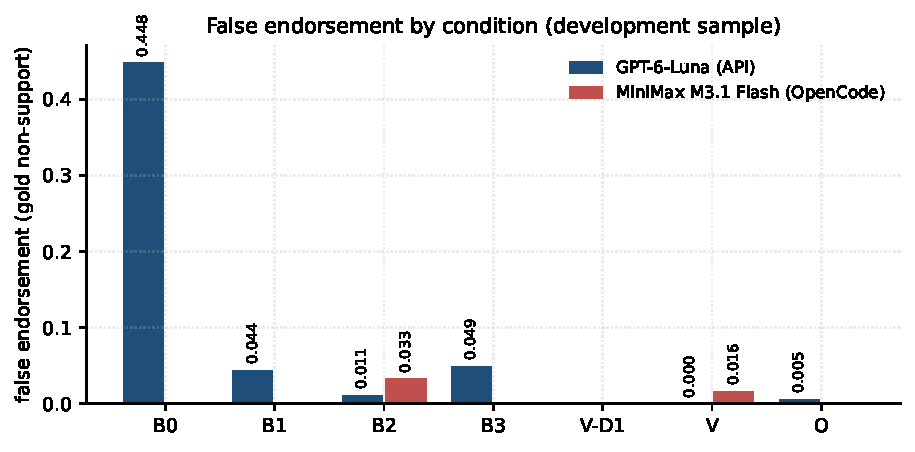
\includegraphics[width=0.82\textwidth]{paper/figures/false_endorsement.pdf}
\caption{False endorsement against SUPPORT recall on the development
sample. B0 (prior knowledge only) is omitted: its false endorsement
(\lunadevBZerofe{}) is an order of magnitude larger. Circles are Luna;
squares are MiniMax.}
\label{fig:falseendorsement}
\end{figure}

The independent-retrieval arm, recovered from V, does not reduce false
endorsement relative to B2. On development, V-D1's rate is
\lunadevVDOnefe{} against B2's \lunadevBTwofe{}. On the held-out
sample it is \lunaheldVDOnefe{} against \lunaheldBTwofe{}: the
independent arm endorses more falsely than the same-evidence baseline.
V's zero false endorsement is therefore a property of the reconciliation
rule, not of retrieval.

\subsection{The class trade-off}

Table~\ref{tab:perclass} breaks the two primary conditions down by
class. V raises SUPPORT precision (from 0.969 to 1.000 on Luna
development) by pushing uncertain claims into NEI, and it pays for that
in SUPPORT recall (\lunadevBTwosupportRecall{} to
\lunadevVsupportRecall{}; 55 missed supports under B2, 66 under V) and
in REFUTE recall (0.790 to 0.627; 13 missed contradictions under B2, 19
under V). MiniMax shows the same shape at a higher absolute level
(\mmdevBTwosupportRecall{} to \mmdevVsupportRecall{}; 17 missed
supports under B2, 36 under V). The cost on the full sample is missed
support first and missed contradiction second. Figure~\ref{fig:failurebreakdown}
makes the Luna counts visible.

\begin{table}[t]
\centering
\caption{Per-class precision, recall, and F1 on the development sample,
with confusion counts. Luna is the frozen-configuration run.}
\label{tab:perclass}
\begin{tabular}{llrrrrrrr}
\toprule
Model family & Method & class & P & R & F1 & TP & FP & FN \\
\midrule
GPT-6-Luna (API) & B2 & SUPPORT & 0.971 & 0.573 & 0.720 & 67 & 2 & 50 \\
GPT-6-Luna (API) & B2 & REFUTE & 0.803 & 0.790 & 0.797 & 49 & 12 & 13 \\
GPT-6-Luna (API) & B2 & NEI & 0.635 & 0.893 & 0.742 & 108 & 62 & 13 \\
\addlinespace[2pt]
GPT-6-Luna (API) & V & SUPPORT & 1.000 & 0.427 & 0.599 & 50 & 0 & 67 \\
GPT-6-Luna (API) & V & REFUTE & 0.949 & 0.597 & 0.733 & 37 & 2 & 25 \\
GPT-6-Luna (API) & V & NEI & 0.564 & 0.983 & 0.717 & 119 & 92 & 2 \\
\addlinespace[2pt]
MiniMax M3.1 Flash (OpenCode) & V & SUPPORT & 0.961 & 0.718 & 0.822 & 74 & 3 & 29 \\
MiniMax M3.1 Flash (OpenCode) & V & REFUTE & 0.933 & 0.792 & 0.857 & 42 & 3 & 11 \\
MiniMax M3.1 Flash (OpenCode) & V & NEI & 0.719 & 0.960 & 0.822 & 97 & 38 & 4 \\
\addlinespace[2pt]
\bottomrule
\end{tabular}

\end{table}

\begin{figure}[t]
\centering
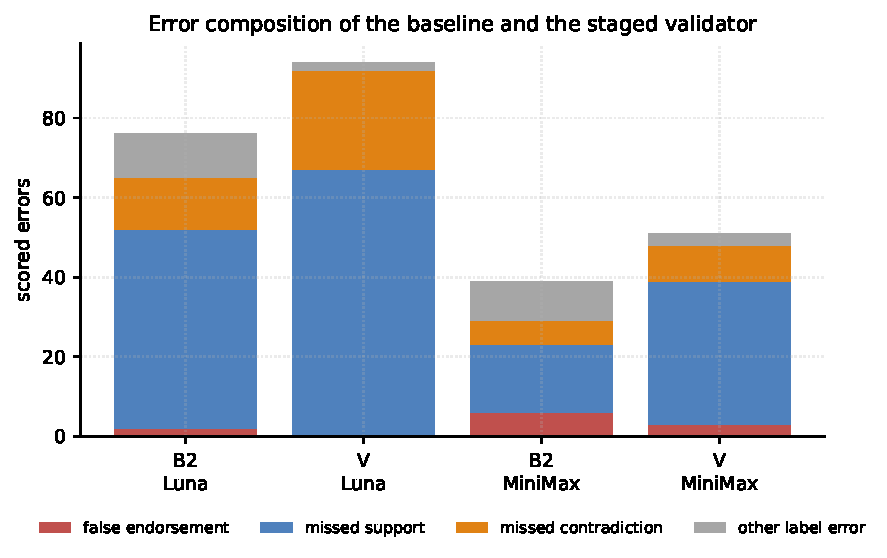
\includegraphics[width=0.82\textwidth]{paper/figures/failure_breakdown.pdf}
\caption{Scored error counts for B2 and V on the frozen development
sample. Execution failures are excluded and counted in
Table~\ref{tab:sensitivity}.}
\label{fig:failurebreakdown}
\end{figure}

\subsection{The 2$\times$2 cells}

Table~\ref{tab:ablation} separates evidence access from reading policy
as far as the condition matrix allows. The cells are not a clean
factorial: they differ in what the final step sees and in the label
space, and V-D1 is derived from V. Read as a descriptive grid, two
patterns appear under Luna. Claim-visible judging beats evidence-first
judging on micro-F1 (B1 \lunadevBOnemicroFOne{} against B2
\lunadevBTwomicroFOne{}; B3 \lunadevBThreemicroFOne{} against V-D1
\lunadevVDOnemicroFOne{}). Evidence access barely moves the
evidence-first cell (V-D1 FE \lunadevVDOnefe{} against B2
\lunadevBTwofe{}). MiniMax does not repeat the claim-visible advantage
(B1 \mmdevBOnemicroFOne{} against B2 \mmdevBTwomicroFOne{}) and did not
complete B0, B3, or O. We therefore treat the grid as a Luna-development
description, not as a replicated factorial.

\begin{table}[t]
\centering
\caption{Condition grid on the development sample. V-D1 is derived from
the V predictions, not re-run.}
\label{tab:ablation}
\begin{tabular}{llrrrr}
\toprule
Model family & Cell & Evidence & Reading policy & micro-F1 & FE (gold non-sup) \\
\midrule
GPT-6-Luna (API) & B0 & none & prior knowledge & 0.547 & 0.448 \\
GPT-6-Luna (API) & B1 & D0 & claim-visible & 0.843 & 0.044 \\
GPT-6-Luna (API) & B2 & D0 & neutral / evidence-first & 0.747 & 0.011 \\
GPT-6-Luna (API) & B3 & D1 & claim-visible & 0.800 & 0.049 \\
GPT-6-Luna (API) & V-D1 & D1 & neutral / evidence-first & 0.757 & 0.016 \\
GPT-6-Luna (API) & V & D0 $\cup$ D1 & reconciled & 0.687 & 0.000 \\
GPT-6-Luna (API) & O & gold rationales & claim-visible & 0.870 & 0.005 \\
\addlinespace[2pt]
MiniMax M3.1 Flash (OpenCode) & B2 & D0 & neutral / evidence-first & 0.870 & 0.033 \\
MiniMax M3.1 Flash (OpenCode) & V-D1 & D1 & neutral / evidence-first & 0.853 & 0.033 \\
MiniMax M3.1 Flash (OpenCode) & V & D0 $\cup$ D1 & reconciled & 0.830 & 0.016 \\
\addlinespace[2pt]
\bottomrule
\end{tabular}

\end{table}

\subsection{Where the abstentions come from}
\label{sec:mechanism}

V stores its four-way label alongside the mapped native label. On the
frozen development sample it predicts NEI on \lunadevVlabelsnei{} of
\lunadevVlabelstotal{} claims, of which \lunadevVlabelsunaddressed{} are
unaddressed and \lunadevVlabelsunderdetermined{} are underdetermined
(Figure~\ref{fig:labels}). SciFact's gold cannot score that split.

\begin{figure}[t]
\centering
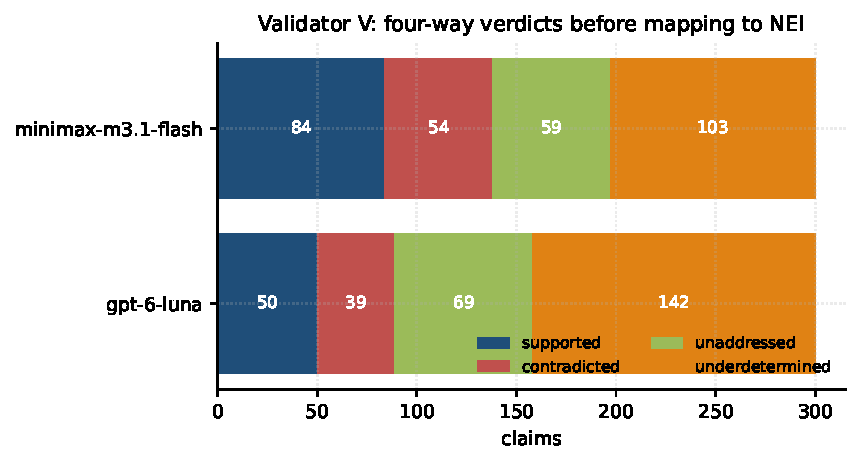
\includegraphics[width=0.62\textwidth]{paper/figures/label_distribution.pdf}
\caption{V's four-way verdicts on the frozen development sample, before
the mapping onto SciFact's three-way label space.}
\label{fig:labels}
\end{figure}

The more informative split is whether the two scopes agreed.
Table~\ref{tab:mechanism} conditions accuracy on that split, now
separated into three groups: the same four-way label; both no-verdict
labels (unaddressed versus underdetermined, both NEI); and a genuine
disagreement on the scored three-way label. When the four-way labels
agree, V matches B2 (\lunadevAgreeVacc{} against
\lunadevAgreeBTwosAcc{} on \lunadevAgreeN{} development claims). When
both scopes already say NEI in different words
(\lunadevNeiOnlyN{} claims), V abstains and is right about as often as
B2 (\lunadevNeiOnlyVacc{} against \lunadevNeiOnlyBTwosAcc{}). When the
scored labels differ (\lunadevConflictN{} claims), V abstains on every
claim by construction and is right on \lunadevConflictVacc{} of them;
B2 is right on \lunadevConflictBTwosAcc{}. The held-out sample is
sharper: B2 is right on \lunaheldConflictBTwosAcc{} of the
\lunaheldConflictN{} three-way conflicts, V on
\lunaheldConflictVacc{}. ``Disagreement drives abstention'' is the
algorithm. The empirical content is that the conflict signal is a weak
predictor of a B2 error.

\begin{table}[t]
\centering
\caption{Accuracy conditioned on the two evidence scopes. ``Both no
verdict'' means the four-way labels differ but both map to NEI.
``Different scored label'' means SUPPORT, REFUTE, and NEI disagree. V
abstains on every row of the last two groups by construction.
Fail-closed rows are excluded.}
\label{tab:mechanism}
\footnotesize
\setlength{\tabcolsep}{5pt}
\begin{tabular}{@{}lrrrr@{}}
\toprule
Scopes & $n$ & B2 acc. & V acc. & V NEI \\
\midrule
\multicolumn{5}{@{}l}{\emph{GPT-6 Luna, development}} \\[1pt]
same four-way label & 163 & 0.828 & 0.828 & 0.540 \\
both no verdict, different kind & 50 & 0.600 & 0.580 & 1.000 \\
different scored label & 55 & 0.618 & 0.309 & 1.000 \\
\midrule
\multicolumn{5}{@{}l}{\emph{GPT-6 Luna, held-out}} \\[1pt]
same four-way label & 139 & 0.871 & 0.842 & 0.496 \\
both no verdict, different kind & 73 & 0.603 & 0.548 & 1.000 \\
different scored label & 50 & 0.700 & 0.100 & 1.000 \\
\midrule
\multicolumn{5}{@{}l}{\emph{MiniMax M3.1 Flash, development}} \\[1pt]
same four-way label & 214 & 0.911 & 0.925 & 0.355 \\
both no verdict, different kind & 36 & 0.861 & 0.917 & 1.000 \\
different scored label & 50 & 0.700 & 0.360 & 1.000 \\
\bottomrule
\end{tabular}

\end{table}

\subsection{Alternative decision rules}

Because V stores both scope labels, alternative reconciliation rules can
be applied without a new model call (Table~\ref{tab:reconcile}). Trusting
\Done{} alone recovers B2's development accuracy (0.743) at a higher
false-endorsement rate (0.019). Trusting \Dzero{}, or falling back from
\Dzero{} to \Done{} when \Dzero{} has no verdict, raises accuracy and
false endorsement together. No saved-label rule is both more accurate
than B2 and lower in false endorsement. On the held-out sample, trusting
\Done{} alone is the cell that produces the \lunaheldVDOnefe{}
false-endorsement rate already noted.

\begin{table}[t]
\centering
\caption{Alternative decision rules applied to the saved per-scope
labels, on claims where both B2 and V completed. No model is called.}
\label{tab:reconcile}
\footnotesize
\setlength{\tabcolsep}{5pt}
\begin{tabular}{@{}lrrrr@{}}
\toprule
Decision rule & accuracy & FE & SUPPORT R & REFUTE R \\
\midrule
\multicolumn{5}{@{}l}{\emph{GPT-6 Luna, development ($n=268$)}} \\[1pt]
B2 baseline (reference) & 0.743 & 0.012 & 0.523 & 0.804 \\
Both scopes must agree (V as run) & 0.675 & 0.000 & 0.383 & 0.627 \\
Citation scope only (D0) & 0.683 & 0.019 & 0.430 & 0.686 \\
Independent scope only (D1) & 0.743 & 0.019 & 0.598 & 0.745 \\
D0, falling back to D1 when D0 has no verdict & 0.750 & 0.037 & 0.645 & 0.804 \\
\midrule
\multicolumn{5}{@{}l}{\emph{GPT-6 Luna, held-out ($n=262$)}} \\[1pt]
B2 baseline (reference) & 0.763 & 0.013 & 0.585 & 0.754 \\
Both scopes must agree (V as run) & 0.618 & 0.000 & 0.368 & 0.456 \\
Citation scope only (D0) & 0.653 & 0.000 & 0.415 & 0.526 \\
Independent scope only (D1) & 0.721 & 0.032 & 0.585 & 0.614 \\
D0, falling back to D1 when D0 has no verdict & 0.756 & 0.032 & 0.632 & 0.684 \\
\midrule
\multicolumn{5}{@{}l}{\emph{MiniMax M3.1 Flash, development ($n=300$)}} \\[1pt]
B2 baseline (reference) & 0.870 & 0.033 & 0.855 & 0.903 \\
Both scopes must agree (V as run) & 0.830 & 0.016 & 0.692 & 0.823 \\
Citation scope only (D0) & 0.847 & 0.038 & 0.769 & 0.919 \\
Independent scope only (D1) & 0.853 & 0.033 & 0.829 & 0.823 \\
D0, falling back to D1 when D0 has no verdict & 0.873 & 0.055 & 0.906 & 0.919 \\
\bottomrule
\end{tabular}

\end{table}

\subsection{Evidence acquisition}

Table~\ref{tab:retrieval} reports what independent retrieval bought.
Recall@$k$ is \retrievalRecall{} over the \retrievalNAnnotated{} claims
that have annotated evidence, but every annotated document it finds was
also cited: unique yield is \retrievalUnique{}. In SciFact the cited
document set contains the annotated document set, so a retriever that
searches the same corpus cannot find new gold evidence. It can only add
unannotated context, and \retrievalUnjudged{}\% of what it returns is
unjudged. The independent arm therefore cannot repair a wrong citation
on this corpus, because a wrong citation is, by construction, a document
without a rationale. That property bounds every claim in this paper. The
experiment that would test the motivating hypothesis---swap \Dzero{} for
non-gold abstracts and ask whether \Done{} recovers the gold
rationale---was not run.

\begin{table}[t]
\centering
\caption{Evidence acquisition for the independent-retrieval arm on the
development sample.}
\label{tab:retrieval}
\begin{tabular}{lr}
\toprule
Quantity & Value \\
\midrule
Claims scored & 300 \\
Claims with annotated evidence & 179 \\
Passages retrieved per claim ($k$) & 8 \\
Recall@$k$ (annotated documents found) & 0.849 \\
Precision@$k$ (retrieved documents annotated) & 0.074 \\
Overlap with $D_0$ (retrieved documents also cited) & 0.096 \\
Unique yield (annotated found but not cited) & 0.000 \\
Refuting yield (contradicting documents found) & 0.171 \\
Unjudged rate (no annotation) & 0.926 \\
Retrieved documents & 2400 \\
Annotated documents retrieved that were not cited & 0 \\
\bottomrule
\end{tabular}

\end{table}

\subsection{A second model and a thirty-claim subset}

MiniMax M3.1 Flash, reached through a different harness, reproduces the
direction of the V-versus-B2 contrast on the development sample
(Table~\ref{tab:paired}): V is more conservative, SUPPORT recall falls,
and the McNemar test does not reject. MiniMax is a markedly better
verifier in absolute terms (B2 micro-F1 \mmdevBTwomicroFOne{} against
\lunadevBTwomicroFOne{}). The two models are not matched for size,
training, or harness, and MiniMax has no held-out run and an incomplete
condition matrix (B0, B3, O, and calibration never completed: the free
endpoint that served it was withdrawn). It corroborates the specified
contrast, not the wider grid.

To check whether the conservative shift belongs only to these two
models we repeated B2 versus V on a frozen thirty-claim subset with
\sweepModelsWord{} closed-weight models from one vendor lineage,
including Luna (Table~\ref{tab:sweep}, Figure~\ref{fig:modelsweep}).
Thirty claims can resolve a difference of several claims, not a
one-point false-endorsement rate; every $\Delta$FE interval collapses
to $[0,0]$. What the subset can show is where a shift lands: REFUTE
recall falls under V in \sweepRefuteLowerPhrase{}, while SUPPORT recall
is unchanged in \sweepSupportEqualWord{} of the four. That concentration
does not match the full-sample class breakdown
(Table~\ref{tab:perclass}), so the subset is a directional check on a
handful of claims, not a finding about the cost of staging.

\begin{table}[t]
\centering
\caption{B2 versus V on the frozen thirty-claim subset. Cells after the
interval are ``B2 / V''. The subset is descriptive: read it for
direction, not for significance. All four models are closed-weight
models from one vendor lineage; Luna is the primary model, not a
held-out replicate.}
\label{tab:sweep}
\scriptsize
\setlength{\tabcolsep}{5pt}
\begin{tabular}{@{}llrrrr@{}}
\toprule
Model & Weights & $\Delta$FE [95\% CI] & SUPPORT R & REFUTE R & micro-F1 \\
\midrule
GPT-6 Astra & closed & +0.000 [0.000, 0.000] & 0.700 / 0.600 & 0.900 / 0.500 & 0.833 / 0.700 \\
GPT-6 Sol & closed & +0.000 [0.000, 0.000] & 0.700 / 0.700 & 0.800 / 0.500 & 0.833 / 0.733 \\
GPT-5.6 Terra & closed & +0.000 [0.000, 0.000] & 0.700 / 0.700 & 0.900 / 0.500 & 0.867 / 0.733 \\
GPT-6 Luna & closed & +0.000 [0.000, 0.000] & 0.500 / 0.500 & 0.900 / 0.500 & 0.800 / 0.667 \\
\bottomrule
\end{tabular}

\end{table}

\begin{figure}[t]
\centering
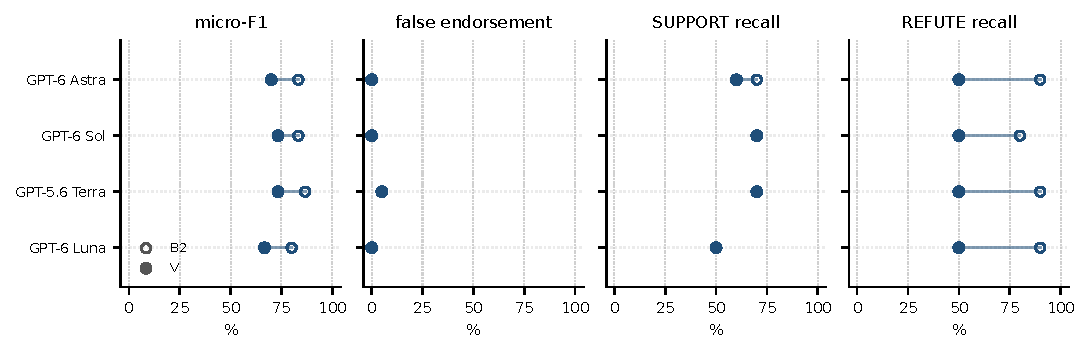
\includegraphics[width=\textwidth]{paper/figures/model_sweep.pdf}
\caption{B2 to V on the thirty-claim subset. Hollow marks are B2, filled
marks are V. The largest false-endorsement rate in any row is
\sweepFEmaxPct{}.}
\label{fig:modelsweep}
\end{figure}

\subsection{Cost}

Table~\ref{tab:cost} reports model calls and measured tokens for Luna,
now taken from the same development run for every condition. V issues
three calls per claim against B2's two. A B2 call measures about
\lunadevBTwoTokensPerCall{} tokens and a V call about
\lunadevVTokensPerCall{}, so V costs about \lunaTokenRatio{} times B2
per claim. In exchange V produces two scoped judgments instead of one.
A deployment that only needs a single verdict is better served by B2;
the value of V is that its two scopes are separately auditable. MiniMax
has no cost row: its harness preamble dominates every prompt.

\begin{table}[t]
\centering
\caption{Calls per claim and measured tokens for GPT-6 Luna, taken from
the development run that recorded the most calls for each condition.
Estimated tokens per claim is the product of the two preceding columns.
Resumed runs keep only the last invocation's usage record, so this is
an estimate, not a per-claim total.}
\label{tab:cost}
\footnotesize
\setlength{\tabcolsep}{5pt}
\begin{tabular}{@{}llrrrr@{}}
\toprule
Split & Method & tokens/claim & calls/claim & median (s) & p95 (s) \\
\midrule
\multicolumn{6}{@{}l}{\emph{GPT-6-Luna (API)}} \\[1pt]
dev300 & B0 & 1 & 0.00 & 3.4 & 3.4 \\
dev300 & B1 & 749 & 1.00 & 2.3 & 5.2 \\
dev300 & B2 & 1,210 & 2.00 & 2.6 & 3.8 \\
dev300 & B3 & 3,064 & 1.00 & 2.6 & 7.9 \\
dev300 & V & 20 & 0.01 & 3.2 & 3.5 \\
dev300 & O & 379 & 1.00 & 2.1 & 5.5 \\
heldout300 & B2 & 1,202 & 2.00 & 17.2 & 21.6 \\
heldout300 & V & 7,431 & 2.86 & 12.5 & 23.7 \\
calibration & B1 & 773 & 1.00 & 3.1 & 4.9 \\
\midrule
\multicolumn{6}{@{}l}{\emph{MiniMax M3.1 Flash (OpenCode)}} \\[1pt]
dev300 & B2 & 0 & 0.00 & --- & --- \\
dev300 & V & 0 & 0.00 & --- & --- \\
\bottomrule
\end{tabular}

\end{table}

\subsection{Fail-closed rows and the second development run}
\label{sec:second-run}

Table~\ref{tab:sensitivity} repeats B2 and V under both accountings.
On the frozen development run, scoring V's \lunadevVfailclosed{}
fail-closed rows as NEI lowers micro-F1 from \lunadevVmicroFOne{} to
\lunadevVallrowsmicroFOne{}; false endorsement stays at zero. Those
\lunadevVfailclosed{} claims are not a random slice: gold is SUPPORT on
\lunadevVfailsupport{}, REFUTE on \lunadevVfailrefute{}, and NEI on
\lunadevVfailnei{}. The held-out run, which also does not retry, lost
\lunaheldVfailclosed{} of 300 claims, of which
\lunaheldVfailsupport{} are gold SUPPORT; all-rows micro-F1 falls from
\lunaheldVmicroFOne{} to \lunaheldVallrowsmicroFOne{}. The runner
overwrites the failure reason at reconcile time, so timeout, parse, and
transport cannot be separated.

The 2026-10-20 development re-run recovered every failed V request and
left V's false endorsement at zero (SUPPORT recall
\lunarerunVsupportRecall{}). It is not interchangeable with the frozen
run: B2 flipped \lunaflipsBTwo{} of \lunaflipsBTwon{} labels
(\lunaflipsBTwopct{}\%) and V flipped \lunaflipsV{} of
\lunaflipsVn{} previously-ok labels (\lunaflipsVpct{}\%) at
temperature 0. The specified contrast (V more conservative, interval
covering zero, McNemar $p=0.50$ on 2 versus 0 pairs) is the same in
both runs.

\begin{table}[t]
\centering
\caption{Sensitivity to the fail-closed accounting and to the second
development run. ``Scored only'' excludes execution failures; ``all
rows'' scores every submitted claim with the label the method recorded.}
\label{tab:sensitivity}
\begin{tabular}{llrrrrr}
\toprule
Model family & Method & accounting & $n$ scored & micro-F1 & FE (gold non-sup) & SUPPORT recall \\
\midrule
GPT-6-Luna (API) & B2 (dev300) & scored only & 300 & 0.747 & 0.011 & 0.573 \\
GPT-6-Luna (API) & B2 (dev300) & all rows & 300 & 0.747 & 0.011 & 0.573 \\
GPT-6-Luna (API) & V (dev300) & scored only & 300 & 0.687 & 0.000 & 0.427 \\
GPT-6-Luna (API) & V (dev300) & all rows & 300 & 0.687 & 0.000 & 0.427 \\
GPT-6-Luna (API) & B2 (heldout300) & scored only & 300 & 0.760 & 0.017 & 0.581 \\
GPT-6-Luna (API) & B2 (heldout300) & all rows & 300 & 0.760 & 0.017 & 0.581 \\
GPT-6-Luna (API) & V (heldout300) & scored only & 262 & 0.618 & 0.000 & 0.368 \\
GPT-6-Luna (API) & V (heldout300) & all rows & 300 & 0.583 & 0.000 & 0.315 \\
\addlinespace[2pt]
MiniMax M3.1 Flash (OpenCode) & V (dev300) & scored only & 257 & 0.829 & 0.019 & 0.718 \\
MiniMax M3.1 Flash (OpenCode) & V (dev300) & all rows & 272 & 0.812 & 0.018 & 0.692 \\
\addlinespace[2pt]
\bottomrule
\end{tabular}

\end{table}

\section{Discussion}

The staged validator did not significantly reduce false endorsement
relative to a baseline that already read the original citations. The
correct reading of that sentence is narrow. The comparison is
underpowered (two discordant events on Luna, five versus two on
MiniMax). The comparison is not compute-matched. The comparison is not
a test of independent retrieval as a repair for bad citations, because
SciFact never presents a bad citation. What the data do show is that
adding a second reader of the same literature, and abstaining when the
two readers disagree, produces a conservative operating point whose
errors are mostly missed support.

Staging is not free of side effects even as a conservative policy. On
the claims where the scored labels differ, B2 is more often right than
the gold-NEI rate that V achieves by abstaining. A reader who treats
every abstention as a signal that the claim is unsupported would be
making a new error; that is why the interface keeps the scientific
verdict (``underdetermined'') separate from the system action (``defer'').

A better decision procedure for the conflict case is the obvious next
step: trust one scope, require three-way rather than four-way
agreement, or hand the conflict to a reader. Table~\ref{tab:reconcile}
shows that none of the saved-label shortcuts is free. The experiment
that would reopen RQ1 is a citation-corruption condition on this
corpus, or a move to SciFact-Open, where independent retrieval can
actually find new evidence.

\section{Limitations}

\begin{itemize}
  \item \textbf{The benchmark cannot test the motivating mechanism.}
    Unique yield is zero by construction. A citation-swap experiment was
    not run.
  \item \textbf{The primary test is underpowered} and the comparison is
    not compute-matched. RQ1's ``matched inference budget'' was not
    implemented.
  \item \textbf{No public preregistration.} The freeze record is an
    internal hash lock written after the development outcome was known.
    The primary development numbers use that frozen configuration; a
    later retry re-run is reported separately.
  \item \textbf{The 2$\times$2 is confounded} by final-step inputs,
    label space, and a derived V-D1 arm.
  \item \textbf{Four-way labels are not human-validated.} The
    unaddressed / underdetermined split is descriptive.
  \item \textbf{One corpus, one domain, abstract-level text.} English
    biomedical abstracts. Claims that need methods, figures, or
    supplements are out of scope.
  \item \textbf{Supplied claims, not generated reports.} The proposer
    is not scored.
  \item \textbf{The two models are not matched}, MiniMax's matrix is
    incomplete, and the thirty-claim subset is four closed-weight
    models from one vendor lineage, including the primary model.
  \item \textbf{SciFact contamination is unchecked} beyond B0
    (SUPPORT recall \lunadevBZerosupportRecall{} from the claim alone).
  \item \textbf{No user study.} See RQ3.
\end{itemize}

\section{Ethics}

The task is interpreting published abstracts, not giving medical
advice. The rendered output is a label, a rationale, and a search
scope; it is not a clinical recommendation. Abstention has its own
risk: a reader who sees an abstention may infer that the claim is
false. Any deployment should display the scientific verdict and the
system action separately. The MiniMax harness is an interactive coding
runtime; we ran it with a fixed preamble, a fixed corpus, and no
tool-enabled tasks.

\section{Conclusion}

A staged, evidence-first validator for scientific claims---a sealed
reader, a claim-visible judge, a citation auditor, and a reconciler
that reports two evidence scopes separately---did not significantly
reduce false endorsement relative to a same-evidence baseline on
SciFact. It became a conservative checker whose errors come mostly
from disagreement between two readers of the same literature, and
whose conservatism is a reconciliation rule rather than a retrieval
gain. Independent retrieval cannot find new gold evidence on this
benchmark. We report that as an inconclusive result, with the
mechanism, the cost, the second run, and the artifact needed to re-run
it. The next step is a decision procedure for scope disagreement, and
an experiment in which the original citations can actually be wrong.

\appendix

\section{Prompts and output contracts}
\label{app:prompts}

The prompts are versioned files under \texttt{prompts/}; the run sidecar
records each file's SHA-256 and the bundle hash. The contracts are:

\begin{quote}
\small
\textbf{Reader (claim-blind).} Input: a neutral question and a list of
passages with identifiers. Output: \texttt{\{"answer": str,
"cited\_doc\_ids": [int]\}}. The reader is not shown the claim, the
asserted answer, the report, or any gold rationale.

\textbf{Judge (claim-visible).} Input: the atomic claim, the sealed
reader record, and the passages. Output: \texttt{\{"label": one of
supported, contradicted, unaddressed, underdetermined;
"rationale\_codes": [str]; "cited\_span\_ids": [str];
"uncertainty\_reasons": [str]\}}.

\textbf{Citation auditor (D0 only).} Input: the atomic claim and the
original cited passages. Output: the judge contract plus
\texttt{\{"citations": [\{"span\_id": str, "adequacy": adequate |
inadequate | unverifiable, "defects": [str]\}]\}}.

\textbf{Compare (B2).} Input: the claim, the neutral question, and the
sealed reader record. Output: \texttt{\{"label": SUPPORT | REFUTE |
NEI, "rationale": str\}}.
\end{quote}

The parsers reject an out-of-set label, a cited identifier that was not
supplied, and a missing mandatory field.

\section{Metric definitions}
\label{app:metrics}

Let $S$ be the set of scored claims, $g_i \in \{\textsc{support},
\textsc{refute}, \textsc{nei}\}$ the gold label, and $p_i$ the predicted
label. The endorsement class is $E=\textsc{support}$.

\begin{align}
\mathrm{FE}_{\text{gold}} &= \frac{|\{i : p_i = E,\ g_i \neq E\}|}{|\{i : g_i \neq E\}|}
&\mathrm{FE}_{\text{pred}} &= \frac{|\{i : p_i = E,\ g_i \neq E\}|}{|\{i : p_i = E\}|}
\end{align}

Micro-F1 pools the confusion matrix over the three classes; macro-F1
averages the three per-class F1 values. Coverage is the fraction of
submitted claims that produced a scored prediction. The paired
bootstrap resamples cited-document families with replacement (2000
resamples). The exact McNemar $p$-value on $b$ and $c$ discordant pairs
is $2\sum_{i=0}^{\min(b,c)}\binom{b+c}{i}\,2^{-(b+c)}$, capped at 1.

\section{Case records}
\label{app:cases}

The three rows below are selected deterministically from the saved
predictions: the first frozen-development claim whose scopes disagreed
on the scored label, the first whose scopes agreed on underdetermined
while B2 and gold said SUPPORT, and the first B2 false endorsement.

\begin{samepage}
\begin{center}
\captionof{table}{Case studies from the frozen development sample.}
\label{tab:cases}
\footnotesize
\setlength{\tabcolsep}{4pt}
\begin{tabular}{@{}>{\raggedright\arraybackslash}p{0.20\textwidth}>{\raggedright\arraybackslash}p{0.09\textwidth}>{\raggedright\arraybackslash}p{0.09\textwidth}>{\raggedright\arraybackslash}p{0.165\textwidth}>{\raggedright\arraybackslash}p{0.325\textwidth}@{}}
\toprule
Case and claim & Gold & B2 & V (D0 / D1) & What the record shows \\
\midrule
\textbf{Scope conflict, abstained}
\newline
\emph{Rapid phosphotransfer rates are correlated with histidine kinase regulator specificity.} & SUPPORT & NEI & NEI (underdetermined / supported) & The independent scope finds support the citation scope does not; the reconciler refuses to choose and abstains. \\[2pt]
\textbf{Baseline false endorsement}
\newline
\emph{Beta-band coherence is enhanced for visible stimuli over invisible stimuli.} & NEI & SUPPORT & NEI (supported / unaddressed) & The baseline endorses from the original citations; the validator abstains, so the endorsement is caught but not replaced. \\[2pt]
\textbf{Coverage loss, scopes agree}
\newline
\emph{ALDH1 expression is associated with poorer prognosis for breast cancer primary tumors.} & SUPPORT & SUPPORT & NEI (underdetermined / underdetermined) & Both scopes call the evidence inconclusive; the validator abstains on a claim the baseline and the gold endorse. \\[2pt]
\bottomrule
\end{tabular}

\end{center}
\end{samepage}

\section{Protocol for the deferred human study}
\label{app:human-study}

No participant was recruited and no ethics review was obtained. The
protocol is recorded so the absence of results is explicit.

\paragraph{Design.} Thirty non-expert adults (a feasible range of
24--36), plus four to six pilot participants, would each see twelve
short, expert-reviewed items. Condition assignment is counterbalanced:
(A) conclusion plus original citations; (B) A plus the validator
verdict; (C) B plus the evidence-linked explanation. Conditions B and C
must use the same system verdict.

\paragraph{Outcomes.} Pre- and post-interface 0--100 judgements that
the conclusion is adequately supported, a four-way evidence-status
choice, one comprehension question, a use-or-defer decision, and
response time. The primary exploratory outcome is the post-interface
Brier score for evidence support comparing C with B.

\section{Reproduction}
\label{app:repro}

\begin{enumerate}
  \item Install the package and its development extras, and verify the
    pinned corpus hash (\path{data/pins/scifact/}).
  \item Start the model endpoint. For Luna, set
    \texttt{OPENAI\_API\_KEY} and \texttt{OPENAI\_MODEL}. For MiniMax,
    start a local agent server and the loopback bridge in
    \path{tools/opencode_bridge.py}.
  \item The frozen-configuration development run is the artifact under
    \path{artifacts/validator_v_dev300} and
    \path{artifacts/same_evidence_b2_dev300}. The 2026-10-20 re-run is
    under \path{artifacts/api/dev300/}. The held-out run is under
    \path{artifacts/held_out/} and requires \texttt{-{}-frozen-final}.
  \item Regenerate every table and figure
    (\path{scripts/paper/make_tables.py},
    \path{scripts/paper/make_figures.py}) and rebuild the PDF
    (\path{scripts/paper/build_pdf.sh}).
\end{enumerate}

Every number in this paper is read from the generated LaTeX fragments
under \path{paper/tables/}. The prose macros in
\path{paper/tables/macros.tex} are generated by the same script.

\bibliographystyle{plainnat}
\bibliography{paper/references}

\end{document}
